There are many life-relevant ways to measure the differences between adult males and females. The wage gap is an oft-cited number: In the fourth quarter of 2016, white women earned 81.1\% as much as white men and black women earned 92.1\% as much as black men. This reveals a gap not only by gender, but also by race with Black (Hispanic) women only earning 67.8\% (62.0\%) as much as white men and black (Hispanic) men earning 73.6\% (71.4\%) as much as white men.\footnote{\citet{USDPTL_2017_Wage_News-Release}.}

 Although this favors males, there are related measures of gender differences that favor females. In both criminal activity and educational attainment, females fare better than males, on average. In 2015, 488 per 100,000 males were incarcerated in comparison to 64 per 100,000 females. When further dividing these statistics by race, the difference between genders and races becomes more stark. While 457 per 100,000 white males were incarcerated, 2,613 (1,043) per 100,000 African-American (Hispanic) males were incarcerated. The rates for females were 52 per 100,000 white females in comparison to 103 (63) per 100,000 African-American (Hispanic) females. In 2012-2013, more females than males received bachelor's degrees across all races with larger disparities for African-American (65\% of the degrees conferred to females) and Hispanics (60\%).

These differences seen as adults are the 

We examine the early-life gender differences of a sample of subjects from disadvantaged families living in Chapel Hill, North Carolina in the 70s and 80s. These subjects were part of two nearly identical studies: the Carolina Abecedarian Project and the Carolina Approach to Responsive Education (ABC/CARE). Those in the treatment group received high-quality, intensive, early childhood education from shortly after birth until entrance into elementary school. Measures of cognitive, social-emotional, and parenting skills were collected on the children during and after the treatment. Figure~\ref{fig:intro-skills-plots} shows the differences between the males and females along these skills.

\begin{sidewaysfigure}
\begin{center}
\caption{Mean Differences between Males and Females, Skills}
\label{fig:intro-skills-plots}
\begin{subfigure}[b]{0.49\textwidth}
	\caption{IQ Measurements}
	\label{fig:intro-skills-plots-cog}
	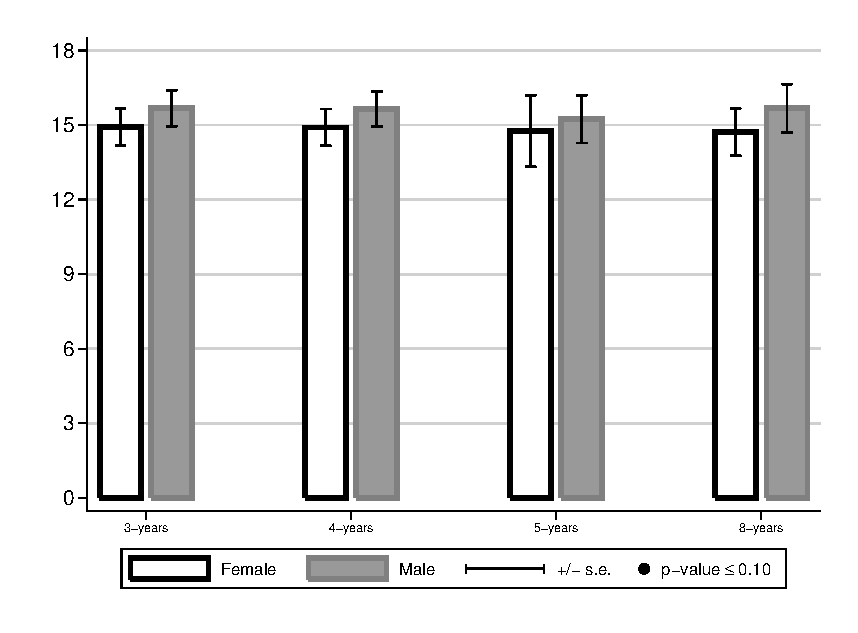
\includegraphics[width=\textwidth]{../output/abccare-gdiff-cog}
\end{subfigure}
\begin{subfigure}[b]{0.49\textwidth}
	\caption{Social-emotional Measurements}
	\label{fig:intro-skills-plots-ncog}
	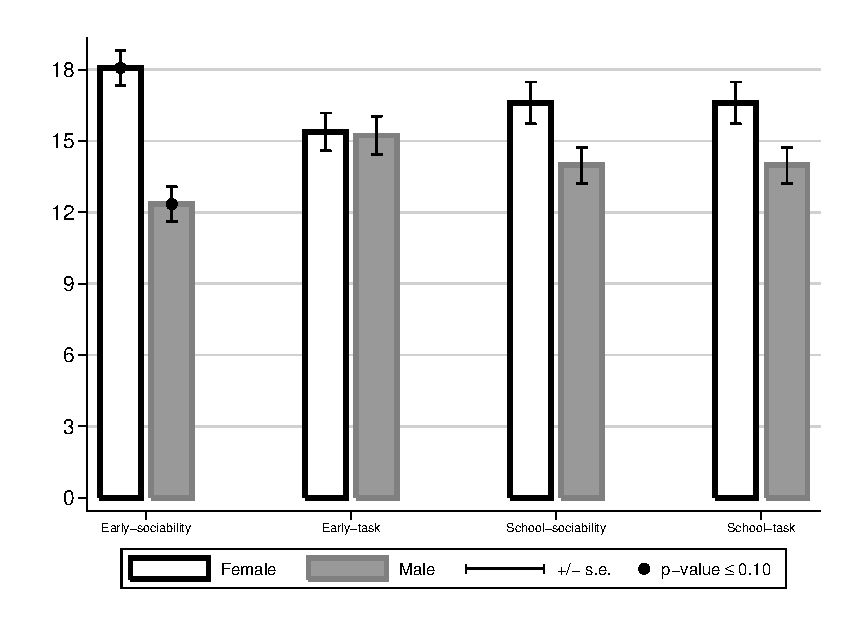
\includegraphics[width=\textwidth]{../output/abccare-gdiff-ncog}
\end{subfigure}

\begin{subfigure}[b]{0.49\textwidth}
	\caption{Achievement Measurements}
	\label{fig:intro-skills-plots-ach}
	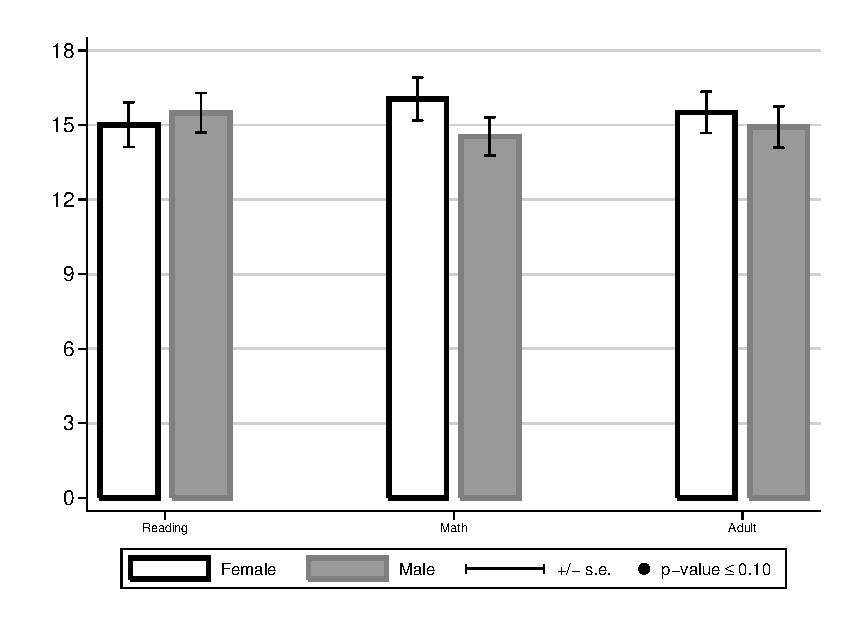
\includegraphics[width=\textwidth]{../output/abccare-gdiff-ach}
\end{subfigure}
\begin{subfigure}[b]{0.49\textwidth}
	\caption{Parenting Measurements}
	\label{fig:intro-skills-plots-parenting}
	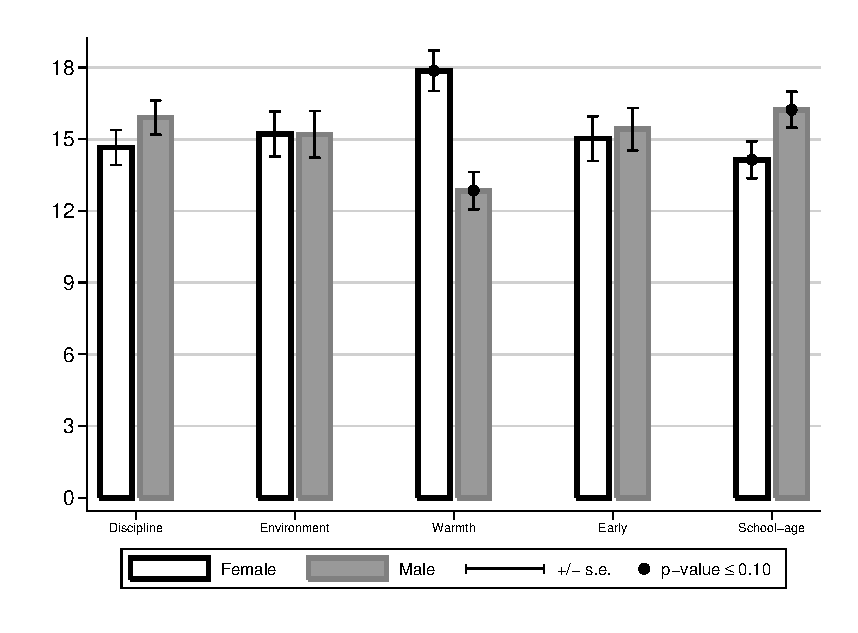
\includegraphics[width=\textwidth]{../output/abccare-gdiff-parenting}
\end{subfigure}
\end{center}
\raggedright \tiny
Note: These plots show the means of factor variables by gender, pooling across experimental groups. All factor variables are calculated by principal factor analysis. The factors are then standardized and divided into 30 quantiles. The IQ factors include different measurements at the specified ages. The social-emotional factors are divided by early (0.5, 1, and 1.5 years) and school-age (6 and 8 years). The scales presented here are sociability and task orientation. The achievement factors are school-age math and reading factors (6, 7.5, 8, 8.5, 9, and 12 years) and an adult factor combining math and reading at 21 years. The parenting factors include factors of the subscales absence of punishment (discipline), environmental factors (environment), and maternal warmth and involvement (warmth). The other factors combine these scales measured when the subjects were toddlers (0.5, 1.5, and 2.5 years) and when they were older (3.5, 4.5, and 8 years).
\end{sidewaysfigure}

Many studies have shown the life-cycle benefits of early education for children from disadvantaged families.\footnote{\citet{Elango_Hojman_etal_2016_Early-Edu}.} Several of these studies separate analysis by gender and find that males and females benefit differently from early childhood education. For example, \citet{Heckman_Moon_etal_2010_QE} and \citet{Garcia_etal_2016_Comp_CBA_Unpublished}, both of which analyze randomized controlled trials with long-term data follow-ups, find that females tend to have more positive effects in education outcomes while males tend to have more positive effects in labor market and health outcomes. Other studies analyzing programs with shorter-term data also find gender differences in early skills and academic outcomes.\footnote{\citet{Deming_2009_AEJAE} and \citet{Ou_Reynolds_2010_Mechanisms_CYSR} are examples of this.} 

These gender results are variable across studies, however, obfuscating the conclusions.\footnote{\citet{Magnuson_Kelchen_Duncan_etal_2016_ECRQ} use effect sizes and program characteristics from 23 evaluations of early-life interventions to understand the association between program characteristics and effect sizes by gender. This meta-analysis finds that over the programs used, the most pronounced difference in treatment effects between males and females can be found for outcomes related to schooling, e.g. special education and grade retention. However, most of the programs do not have non-cognitive measures and the varied structure of the evaluations makes the conclusions for gender differences suggestive.} Even within the same program, different approaches to analyzing treatment effects can result in seemingly contradictory conclusions. Using data from the Carolina Abecedarian Project and the Carolina Approach to Responsive Education (ABC/CARE), \citet{Garcia_etal_2016_Comp_CBA_Unpublished} calculate a higher lifetime benefit-cost ratio for males (11.10) than for females (2.45), with these ratios including life-cycle projections of health, crime, and income. According to this analysis, the monetary returns of the program from a social perspective are driven more by males than females, making it appear that males benefit more from the program than do females. However, when looking at the treatment effects unweighted by monetary amounts, there are more positive treatment effects for females for certain categories (see Section~\ref{sec:gdiff}). Unlike the cost-benefit analysis, this aggregate result makes it appear that females benefit more from the program in skills, labor market outcomes, and crime outcomes. Although both of these measures aggregate across outcomes, they lead to seemingly contradictory conclusions on the differential effect of early childhood education.

Understanding the mechanisms of the treatment effects complements the above analyses by explaining and understanding the later-life gender differences seen in both approaches. We address the contradiction by focusing on how early childhood education affects the skill formation process of males and females differently, with these skills in turn affecting other outcomes.\footnote{There is also evidence that the development of males and females differs at this age such that they experience early childhood interventions differently. See \citet{Beeghly-etal_2017_IMHJ,Dayton_2017_IMHJ,Iruka_2017_IMHJ,Schore_2017_IMHJ} for recent findings on the topic of different development of males and females early in life. We consider these findings complementary to our own.}

